\documentclass{article}

% Packages required to support encoding
\usepackage{ucs}
\usepackage[utf8x]{inputenc}
\usepackage{graphicx} 
% Packages required by code

% Packages always used
\usepackage{listings}
\usepackage{hyperref}
\usepackage{xspace}
\usepackage[usenames,dvipsnames]{color}
\hypersetup{colorlinks=true,urlcolor=blue}


\usepackage[framed,numbered,autolinebreaks,useliterate] {mcode}


\usepackage{geometry}
\geometry{letterpaper,textwidth=350pt,textheight=680pt,tmargin=60pt,
            left=72pt,footskip=24pt,headsep=18pt,headheight=14pt}
\usepackage{amsmath}
\usepackage{amssymb}
\usepackage{textcase}
\usepackage{soul}

\newcommand{\mat}[1]{\boldsymbol{#1}}\renewcommand{\vec}[1]{\boldsymbol{\mathrm{#1}}}
\newcommand{\vecalt}[1]{\boldsymbol{#1}}

\newcommand{\conj}[1]{\overline{#1}}

\newcommand{\normof}[1]{\|#1\|}
\newcommand{\onormof}[2]{\|#1\|_{#2}}

\newcommand{\itr}[2]{#1^{(#2)}}
\newcommand{\itn}[1]{^{(#1)}}

\newcommand{\eps}{\varepsilon}
\newcommand{\kron}{\otimes}

\DeclareMathOperator{\diag}{diag}
\DeclareMathOperator{\trace}{trace}
\DeclareMathOperator{\tvec}{vec}

\newcommand{\prob}{\mathbb{P}}
\newcommand{\probof}[1]{\prob\left\{ #1 \right\}}

\newcommand{\pmat}[1]{\begin{pmatrix} #1 \end{pmatrix}}
\newcommand{\bmat}[1]{\begin{bmatrix} #1 \end{bmatrix}}
\newcommand{\spmat}[1]{\left(\begin{smallmatrix} #1 \end{smallmatrix}\right)}
\newcommand{\sbmat}[1]{\left[\begin{smallmatrix} #1 \end{smallmatrix}\right]}

\newcommand{\RR}{\mathbb{R}}
\newcommand{\CC}{\mathbb{C}}

\providecommand{\eye}{\mat{I}}
\providecommand{\mA}{\ensuremath{\mat{A}}}
\providecommand{\mB}{\ensuremath{\mat{B}}}
\providecommand{\mC}{\ensuremath{\mat{C}}}
\providecommand{\mD}{\ensuremath{\mat{D}}}
\providecommand{\mE}{\ensuremath{\mat{E}}}
\providecommand{\mF}{\ensuremath{\mat{F}}}
\providecommand{\mG}{\ensuremath{\mat{G}}}
\providecommand{\mH}{\ensuremath{\mat{H}}}
\providecommand{\mI}{\ensuremath{\mat{I}}}
\providecommand{\mJ}{\ensuremath{\mat{J}}}
\providecommand{\mK}{\ensuremath{\mat{K}}}
\providecommand{\mL}{\ensuremath{\mat{L}}}
\providecommand{\mM}{\ensuremath{\mat{M}}}
\providecommand{\mN}{\ensuremath{\mat{N}}}
\providecommand{\mO}{\ensuremath{\mat{O}}}
\providecommand{\mP}{\ensuremath{\mat{P}}}
\providecommand{\mQ}{\ensuremath{\mat{Q}}}
\providecommand{\mR}{\ensuremath{\mat{R}}}
\providecommand{\mS}{\ensuremath{\mat{S}}}
\providecommand{\mT}{\ensuremath{\mat{T}}}
\providecommand{\mU}{\ensuremath{\mat{U}}}
\providecommand{\mV}{\ensuremath{\mat{V}}}
\providecommand{\mW}{\ensuremath{\mat{W}}}
\providecommand{\mX}{\ensuremath{\mat{X}}}
\providecommand{\mY}{\ensuremath{\mat{Y}}}
\providecommand{\mZ}{\ensuremath{\mat{Z}}}
\providecommand{\mLambda}{\ensuremath{\mat{\Lambda}}}
\providecommand{\mPbar}{\bar{\mP}}

\providecommand{\ones}{\vec{e}}
\providecommand{\va}{\ensuremath{\vec{a}}}
\providecommand{\vb}{\ensuremath{\vec{b}}}
\providecommand{\vc}{\ensuremath{\vec{c}}}
\providecommand{\vd}{\ensuremath{\vec{d}}}
\providecommand{\ve}{\ensuremath{\vec{e}}}
\providecommand{\vf}{\ensuremath{\vec{f}}}
\providecommand{\vg}{\ensuremath{\vec{g}}}
\providecommand{\vh}{\ensuremath{\vec{h}}}
\providecommand{\vi}{\ensuremath{\vec{i}}}
\providecommand{\vj}{\ensuremath{\vec{j}}}
\providecommand{\vk}{\ensuremath{\vec{k}}}
\providecommand{\vl}{\ensuremath{\vec{l}}}
\providecommand{\vm}{\ensuremath{\vec{l}}}
\providecommand{\vn}{\ensuremath{\vec{n}}}
\providecommand{\vo}{\ensuremath{\vec{o}}}
\providecommand{\vp}{\ensuremath{\vec{p}}}
\providecommand{\vq}{\ensuremath{\vec{q}}}
\providecommand{\vr}{\ensuremath{\vec{r}}}
\providecommand{\vs}{\ensuremath{\vec{s}}}
\providecommand{\vt}{\ensuremath{\vec{t}}}
\providecommand{\vu}{\ensuremath{\vec{u}}}
\providecommand{\vv}{\ensuremath{\vec{v}}}
\providecommand{\vw}{\ensuremath{\vec{w}}}
\providecommand{\vx}{\ensuremath{\vec{x}}}
\providecommand{\vy}{\ensuremath{\vec{y}}}
\providecommand{\vz}{\ensuremath{\vec{z}}}
\providecommand{\vpi}{\ensuremath{\vecalt{\pi}}}

\sodef\allcapsspacing{\upshape}{0.15em}{0.65em}{0.6em}%

\makeatletter
\def\maketitle{%
\par
\hrule height 0.75pt\vspace{1ex}
\par\noindent
\begin{minipage}{0.5\textwidth}
\scshape
purdue university $\cdot$ CS 580 \\
Introduction to the Analysis of Algorithms
\end{minipage}
\begin{minipage}{0.5\textwidth}
\raggedleft
\MakeTextUppercase{\allcapsspacing{\@title}}\\[0.2ex]
\textit{\@author}\\[0.2ex]
\textit{\@date}
\end{minipage}
\par\vspace{1ex}
\hrule height 1pt
\vspace{2ex}
\par
}
\makeatother

\author{Jun Cheng}
\title{Lecture Notes}
% auto generate a title
\AtBeginDocument{\maketitle}


\title{Homework}



\begin{document} 


\subsection*{Problem 1: }

\begin{align*} 
f(x_1, x_2) &= x_1^3 + 2x_1x_2 - 3x_1^2x_2^2 \\
\frac{df}{dx_1} &= 2x_1^2 + 2x_2 - 6x_1x_2^2 \\
\frac{df}{dx_2} & = 2x_1 -6x_1^2x_2   \\
f_{x_1x_1} & = 4x_1 -6x_2^2 \\
f_{x_1x_2} & = 2 - 12x_1x_2  \\
f_{x_2x_1} & = 2 - 12x_1x_2  \\
f_{x_2x_2} & = -6x_1^2 \\
\end{align*}

Tylor expansion: \\
\begin{align*} 
f(\vx) = f(\vx^0) + (\vx-\vx^0)^T\bigtriangledown f(\vx^0) + (\vx-\vx^0)^TH(\vx)(\vx-\vx^0) \\
\end{align*} 
where $\vx^0 = \bmat{1 \\ 1 }  $ \\
For linear approximation: 

\begin{align*} 
l(x_1, x_2) &  =  f(\vx^0) + (\vx-\vx^0)^T\bigtriangledown f(\vx^0) \\
& = f\left( \bmat{1\\ 1} \right) + \bmat{x_1-1 & x_2-1}\bmat{-1\\-4} \\
& = -x_1 -4x_2 + 5 \\
\end{align*}
Hessian: \\
\begin{align*} 
H = \bmat{f_{x_1x_1} & f_{x_1x_2} \\  f_{x_2x_1} & f_{x_2x_2} } 
\end{align*} 
For quadratic approximation: 
\begin{align*}
f(\vx) & = f(\vx^0) + (\vx-\vx^0)^T\bigtriangledown f(\vx^0) + (\vx-\vx^0)^TH(\vx)(\vx-\vx^0) \\
& = -x_1 -4x_2 + 5 + \bmat{x_1-1 & x_2 -1}\bmat{4x_1 -6x_2^2 & 2 - 12x_1x_2 \\ 2 - 12x_1x_2 & -6x_1^2 } \bmat{x_1-1 \\ x_2 -1 }   \\
& = -x_1 -4x_2 + 5  + (2x_1 - 6x_1^2x_2)(x_1-1)^2 - 6x_1^2(x_2-1)^2 + (4-24x_1x_2)(x_1-1)(x_2-1) \\ 
\end{align*}

\subsection*{Problem 2: } 

\begin{enumerate} 
\item  
\begin{align*}
f(\vx)  & = \bmat{x_1 & x_2} \bmat{1 & 4 \\ 2 & 3} \bmat{x_1 // x_2} - \bmat{x_1 & x_2} \bmat{-2 \\ 1} + \pi \\ 
& = x_1^2 +3 x_2^2 + 6x_1x_2 + 2x_1 + x_2 + \pi \\
\frac{df}{dx_1} &= 2x_1 + 6x_2 + 2 \\
\frac{df}{dx_2} &= 6x_2 + 6x_1 + 1 \\
Df(\vx) &= \bmat{\frac{df}{dx_1} & \frac{df}{dx_2}} = \bmat{2x_1 + 6x_2 + 2 &   6x_2 + 6x_1 + 1} 
\end{align*} 
\item 
\begin{align*} 
f(\vx) & = \frac{1}{2} \bmat{x_1 & x_2 } \bmat{2 & 3 \\ 9 & 1} \bmat{x_1\\ x_2} + \bmat {x_1 & x_2} \bmat {2 \\ -3 }  + \log{3}  \\
& = x_1^2 +  \frac{1}{2}x_2^2 + 6x_1x_2  + 2x_1 - 3x_2 + \log{3} \\ 
\frac{df}{x_1} & = 2x_1 + 6x_2 + 2 \\
\frac{df}{x_2} & = x_2+6x_1 - 3 \\
f_{x_1x_1} &  = 2 \\ 
f_{x_1x_2} &  = 6 \\ 
f_{x_2x_1} &  = 6 \\ 
f_{x_2x_2} &  = 1 \\ 
\end{align*}
Hessian: \\
\begin{align*} 
H = \bmat{2 & 6 \\ 6 & 1} 
\end{align*} 
\end{enumerate} 


\subsection*{Problem 3: } 

\begin{align*} 
f(x_1, x_2) = e^{3x_1x_2^2} 
\end{align*} 
\begin{enumerate} 
\item 
\begin{align*} 
\frac{df}{x_1} &= 3x_2^2e^{3x_1x_2^2}\\
\frac{df}{x_2} &= 6x_1x_2e^{3x_1x_2^2}\\ 
\end{align*} 
Then the gradient at $\vx = \bmat{1 \\ 1} $ is : \\
\begin{align*}
\bmat{3e^3 \\ 6 e^3 } 
\end{align*} 

\item 
Rate of increase of $f$ at the point $\vx=\bmat{1\\1} $  in the direction $\vd$ 
\begin{align*} 
\frac{Df(\vx)\cdot \vd}{\| \vd \|} = \frac{15e^3}{\sqrt{5}} 
\end{align*} 

\item 
In the direction $\vd = \bmat{3 \\ 6 }$, we can have the maximum rate of increase $3\sqrt{5} e^3$ 


\end{enumerate} 


\subsection*{Problem 4: } 
\begin{align*} 
f(x_1, x_2, x_3) &  =  -( x_1^2 + 4\epsilon x_2^2 + 5 x_3^2 -2x_1x_3 + 2\epsilon x_1x_2 + 4 x_2 x_3 )   \\
& =- \bmat{x_1 & x_2 & x_3 } \bmat{1 & \epsilon & -1 \\ \epsilon & 4\epsilon & 2 \\ -1 & 2 & 5} \\
\end{align*}
%Eigenvalues of $ \bmat{1 & \epsilon & -1 \\ \epsilon & 4\epsilon & 2 \\ -1 & 2 & 5} $  are: \\
Using principal minor method: \\ 
\begin{align*} 
k= 1: \\
D_1 &= 20\epsilon - 4 > 0 \\
D_2 &= 7 \\
D_3 &= 4\epsilon - \epsilon^2 >0 \\
k=2 : \\
D_1 &= 1 \\
D_2 &= 4\epsilon>0  \\
D_3 &= 5 \\
k= 3 : \\
D &= 12\epsilon - 4 -5 \epsilon^2 > 0 \\
\end{align*} 

To make the function be negative semi-definite, the range of $\epsilon$ is $ 0.4 \leq \epsilon \leq 2 $ 

\subsection*{Problem 5: } 
\begin{enumerate} 
\item
\begin{align*}
f(x_1, x_2) & = \frac{1}{3}x_2^3 + \frac{1}{2}x_2^2 + 2x_1x_2 + \frac{1}{2}x_1^2-x_1+10 \\
\frac{df}{dx_1} &= 2x_2 + x_1 -1 = 0 \\
\frac{df}{dx_2} &= x_2^2 +x_2 + 2x_1 = 0 \\
\end{align*} 
We can get two points $(-1, 1)$ and $(-3, 2)$ which satisfy the first-order necessary conditions for the extremum. \\
\item 
\begin{align*} 
\frac{df}{dx_1dx_1} &= 1 \\
\frac{df}{dx_1dx_2} &=  2 \\
\frac{df}{dx_2dx_1} &= 2 \\
\frac{df}{dx_2dx_2} &= 2x_2 + 1 \\
\end{align*}
Then Hessian is : \begin{align*} \bmat{1 & 2 \\ 2 & 2x_2 + 1} \end{align*} \\
For point $(-1, 1)$ , \\
$H = \bmat {1 & 2 \\ 2 & 3} $  is indefinite
For point $(-3, 2) $ , \\
$H = \bmat{1 & 2 \\ 2 & 5} $ is positive definite. \\
Then the point $(-3, 2)$ is a strict local minimizer. 

\end{enumerate} 

\subsection*{Problem 6: } 
\begin{align*} 
f(\vx) & = \vx^T\bmat{1 & 0 \\ 1 & 1 } \vx \\
& = x_1^2 + x_1x_2 + x_2^2 \\
\end{align*} 
The direction of travel is:  \\
\begin{align*} 
\vd = -\vg = -\frac{df}{d\vx} = (\mA + \mA^T) \vx = -\bmat{2 & 1 \\ 1 & 2 } \vx  = \bmat{-2x_1-x_2 \\ -x_1-2x_2}\\
\end{align*} 
when $ \epsilon_1  = 0.1;  f(x^{(0)} )= 1.065 $ \\
\begin{align*} 
\vx^{(1)} &= \vx^{(0)} + \epsilon_1 \cdot \vd    \\
	& = \bmat{0.55 \\ 0.55} 
\end{align*} 
when $ \epsilon_2  = 0.2 ; f(x^{(1)} )= 1.65    $\\
\begin{align*} 
\vx^{(2)} & = \vx^{(1)} + \epsilon_2 \cdot \vd    \\
	& = \bmat{-0.11 \\ -0.11} 
\end{align*} 

\subsection*{Problem 7: } 
See Table 1 for  Golden Section search. 
\begin{table}[]
\centering
\caption{Problem 7 Golden section search.}
\label{my-label}
\begin{tabular}{llllll}
k & $a_k$    & $b_k$    & f($a_k$) & f($b_k$) & New interval \\
1 & -0.3    & -0.14   & 0.27    & 0.0588  & 0.576      \\
2 & -0.14   & -0.0457 & 0.0588  & 0.006   & 0.356        \\
3 & -0.0407 & 0.0137  & 0.006   & 000056  & 0.22       \\
4 & 0.0137  & 0.05    & 0.00056 & 0.0075  & 0.135        \\
5 & 0.009   & 0.0137  & 0.0002  & 0.0006  & 0.083       
\end{tabular}
\end{table}



\subsection*{Problem 8: } 
See Table 2 for Fibonacci search. 

\begin{table}[]
\centering
\caption{Problem 8:  Fibonacci search}
\label{my-label}
\begin{tabular}{llllll}
k & $a_k$   & $b_k$  & f($a_k$) & f($b_k$) & New interval \\
1 & -0.42  & -0.19 & 0.53    & 0.108   & 0.58         \\
2 & -0.2   & -0.05 & 0.12    & 0.0075  & 0.36         \\
3 & -0.056 & 0.016 & 0.009   & 0.0007  & 0.072       
\end{tabular}
\end{table}

For Newton Method :\\
\begin{align*} 
f(x) & = 3x^2\\
f'(x) & = 6x\\
f"(x) & = 6\\
\frac{f'(x)}{f"(x)} &= x\\
\end{align*} 
Therefore, we can pick up a random staring point within the initial range, then one step would be enough for a quadratic equation.
\begin{align*} 
x^{(0)} &= 0.46 \\
x^{(1)} & = x^{(0)} - \frac{f'(x^{(0)})}{f"(x^{(0)})} \\
& = 0.46 - 0.46 \\
& = 0 \\
x^{(2)} & = x^{(1)} - \frac{f'(x^{(1)})}{f"(x^{(1)})} \\
& = 0 \\
\end{align*} 

\subsection*{Problem 9: } 
\begin{lstlisting} 
[X, Y] = meshgrid(-1:0.1:1, -1:0.1:1); 
Z = (X-Y).^4 + 12*X.*Y - Y + X + 5; 
mesh(X, Y, Z) ; 
contour(X, Y, Z, 20 ) ; 
%xlabel(X1) ; 
%ylabel(X2); 
box on;
\end{lstlisting} 

\begin{figure} 
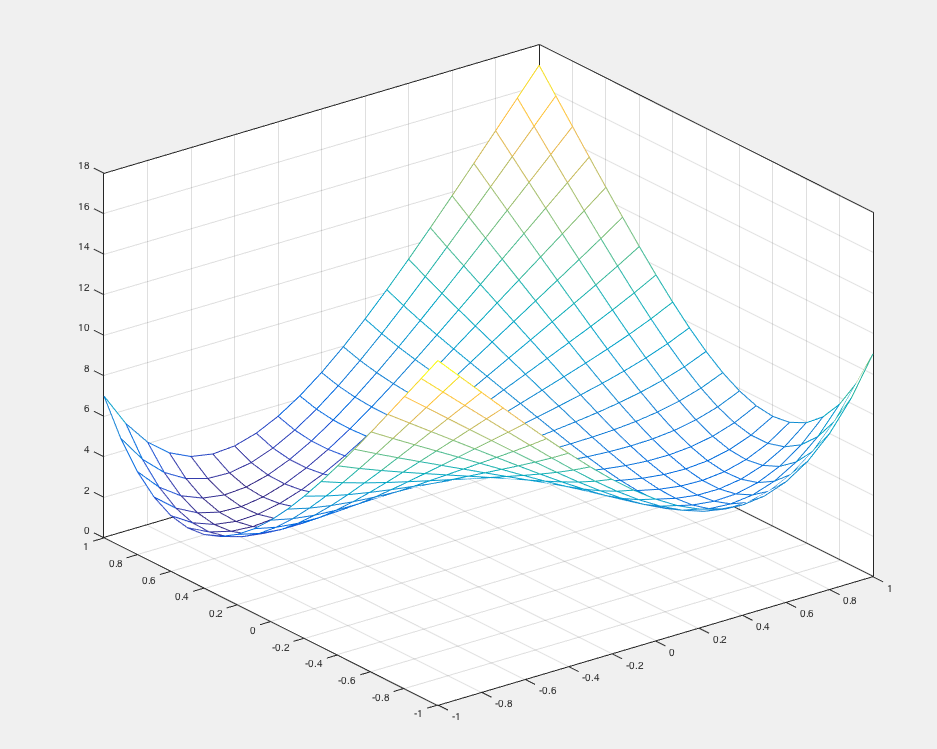
\includegraphics[width=0.5\textwidth]{mesh} 
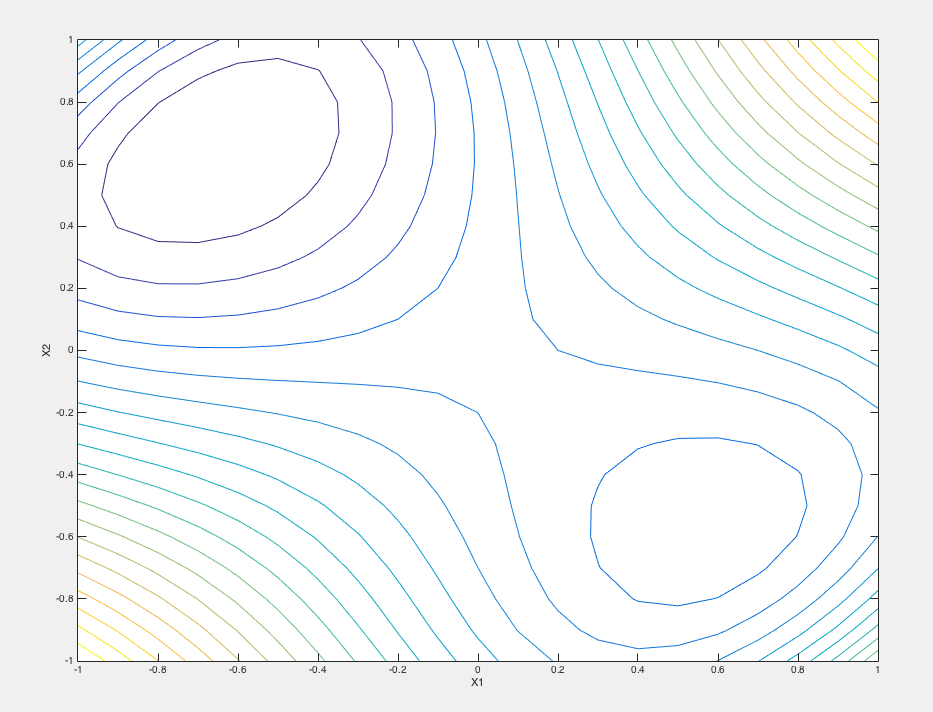
\includegraphics[width=0.5\textwidth]{contour} 

\caption{Left: Problem 9(a) Mesh plot . Right: Problem 9(b) Contour plot. } 

\end{figure} 



\end{document}

